\documentclass[onecolumn]{IEEEtran}
\IEEEoverridecommandlockouts
% The preceding line is only needed to identify funding in the first footnote. If that is unneeded, please comment it out.
\usepackage{cite}
\usepackage{amsmath,amssymb,amsfonts}
\usepackage{algorithmic}
\usepackage{graphicx}
\usepackage{textcomp}
\usepackage{xcolor}
\usepackage{amsmath,amsfonts,amsthm,amssymb}
\usepackage{setspace}
\usepackage{Tabbing}
\usepackage{enumitem}
\usepackage{fancyhdr}
\usepackage{lastpage}
\usepackage{extramarks}
\usepackage[hidelinks]{hyperref}
\usepackage{chngpage}
\usepackage{caption}
\usepackage{subcaption}
\usepackage{soul,color}
\usepackage{float}
\usepackage{graphicx,float,wrapfig}
\usepackage[ruled,vlined]{algorithm2e}
\usepackage{titlesec}
\titleformat{\section}[hang]{\normalfont\large\bfseries}{\thesection}{1em}{}
% code listing settings
\usepackage{listings}
\lstset{
    language=Python,
    basicstyle=\ttfamily\small,
    aboveskip={1.0\baselineskip},
    belowskip={1.0\baselineskip},
    columns=fixed,
    extendedchars=true,
    breaklines=true,
    tabsize=4,
    prebreak=\raisebox{0ex}[0ex][0ex]{\ensuremath{\hookleftarrow}},
    frame=lines,
    showtabs=false,
    showspaces=false,
    showstringspaces=false,
    keywordstyle=\color[rgb]{0.627,0.126,0.941},
    commentstyle=\color[rgb]{0.133,0.545,0.133},
    stringstyle=\color[rgb]{01,0,0},
    numbers=left,
    numberstyle=\small,
    stepnumber=1,
    numbersep=10pt,
    captionpos=t,
    escapeinside={\%*}{*)}
}

\def\BibTeX{{\rm B\kern-.05em{\sc i\kern-.025em b}\kern-.08em
    T\kern-.1667em\lower.7ex\hbox{E}\kern-.125emX}}

% Add page numbers
\fancyhf{} % Clear all headers and footers
\fancyfoot[C]{\thepage} % Footer centered with page number
\renewcommand{\headrulewidth}{0pt} % Remove header rule
\renewcommand{\footrulewidth}{0pt} % Remove footer rule

\pagestyle{fancy} % Enable fancy header/footer

\begin{document}

\title{ECE1512 Project B Report\\Part 2 - LLaVA}

\author{\IEEEauthorblockN{Rémi Grzeczkowicz} \\
\IEEEauthorblockA{\textit{MScAC Student} \\
\textit{University of Toronto - Department of Computer Science}\\
Student Number: 1010905399\\
remigrz@cs.toronto.edu}
}

\maketitle
\thispagestyle{fancy} % Apply fancy header/footer, including the page number on the first page


% \begin{abstract}
% This document is a model and instructions for \LaTeX.
% This and the IEEEtran.cls file define the components of your paper [title, text, heads, etc.]. *CRITICAL: Do Not Use Symbols, Special Characters, Footnotes, 
% or Math in Paper Title or Abstract.
% \end{abstract}

% \begin{IEEEkeywords}
% component, formatting, style, styling, insert
% \end{IEEEkeywords}

For this part, we choose to work on LLaVA designed by \cite{liu2023visualinstructiontuning}.

\section{Summary of the LLaVA model}
LLaVA is a model designed to extend the capabilities of large language models (LLMs) to handle vision-and-language tasks. It achieves this by integrating a vision encoder that processes images into a suitable representation. This image encoding is then concatenated with the textual input and provided as input to the LLM.

\subsection{LLaVA key ideas}
The key ideas of LLaVA are:
\begin{itemize}
    \item \textbf{Multimodal Instruction-Following Data}: LLaVA addresses the challenge of limited vision-language instruction-following data by leveraging GPT-4 to convert image-text pairs into an instruction-following format. This approach generates diverse and high-quality multimodal instruction data, which is essential for effectively training the model.
    \item \textbf{Large Multimodal Model Architecture}: The model integrates the CLIP visual encoder \cite{radford2021learning} with the Vicuna language model \cite{vicuna2023}. This combination enables the model to perform a variety of tasks, including classification, detection, segmentation, and captioning, in an open-world context. The architecture aligns visual features with language embeddings, facilitating seamless interaction between modalities.
    \item \textbf{Instruction Tuning}: LLaVA employs a two-stage instruction-tuning process. First, it pre-trains on a large dataset to align visual and language features. Then, it fine-tunes on task-specific datasets, such as ScienceQA \cite{lu2022learn}, to improve its reasoning capabilities and enhance its ability to follow instructions across various tasks.
    \item \textbf{Evaluation Benchmarks}: To assess its performance, LLaVA introduces two benchmarks: LLaVA-Bench (COCO) \cite{lin2014microsoft}, which evaluates consistency on structured visual inputs, and LLaVA-Bench (In-the-Wild) \cite{githubGitHubComputerVisionintheWildCVinW_Readings}, which challenges the model on diverse and complex tasks. These benchmarks help measure the model’s instruction-following capabilities and its generalization to novel domains.
    \item \textbf{Open Source Contributions}: The project provides open access to its codebase, model checkpoints, and generated multimodal instruction data, fostering further research and development in multimodal AI systems.
\end{itemize}


\subsection{Technical Contributions}
TThe technical contributions of LLaVA are:
\begin{itemize}
    \item \textbf{Introduction of Multimodal Instruction-Following Data}: The authors developed a new pipeline for generating multimodal instruction-following datasets. They transformed image-text pairs into instruction-following formats using symbolic representations (e.g., captions and bounding boxes) and GPT-4. This pipeline produced 158K multimodal samples, including: 58K conversation-based Q\&A, 23K detailed descriptions, and 77K complex reasoning tasks. This innovation addressed the scarcity of high-quality multimodal instruction-following data.
    \item \textbf{Development of Large Multimodal Model Design}: The authors integrated CLIP's visual encoder with Vicuna, an open-source language decoder. They employed a lightweight linear projection layer to map visual features into the language embedding space, enabling efficient alignment. The architecture of the model is illustrated in Figure~\ref{fig:llava_architecture}.
    \item \textbf{Training Approach}: The authors introduced a two-stage tuning process. The first stage involves pre-training on CC3M-derived data to align visual and language features, balancing concept coverage with training efficiency. The second stage focuses on fine-tuning using the generated multimodal datasets for two distinct applications: (1) as a multimodal chatbot, and (2) for scientific Q\&A tasks.
    \item \textbf{Benchmark Design for Multimodal Instruction Following (LLaVA-Bench)}: The authors designed a benchmark to evaluate LLaVA as a multimodal chatbot. This benchmark includes two components: (1) a COCO-based benchmark to test consistency in visual and language instruction alignment using diverse visual content, and (2) an In-the-Wild benchmark to evaluate performance on challenging real-world multimodal tasks, such as memes, sketches, and paintings.
    \item \textbf{State-of-the-Art Performance on ScienceQA}: LLaVA demonstrated state-of-the-art performance on the ScienceQA dataset, which requires reasoning over scientific text and images. This highlights the model’s ability to generalize to novel domains and perform complex multimodal reasoning tasks.
\end{itemize}

\begin{figure}[H]
    \centering
    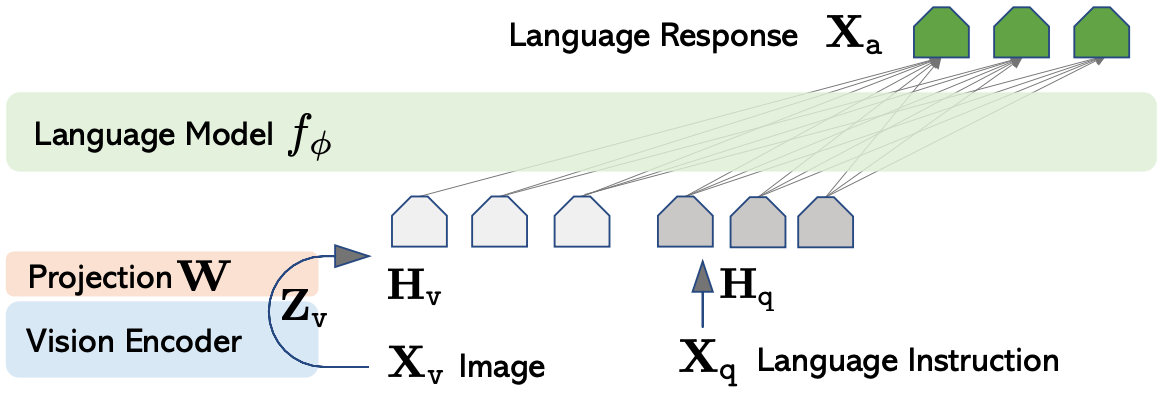
\includegraphics[width=0.8\textwidth]{images/llava_architecture.png}
    \caption{LLaVA architecture}
    \label{fig:llava_architecture}
\end{figure}

\subsection{Areas for Improvement}
The authors suggest several areas for improvement:
\begin{itemize}
    \item \textbf{Hallucination and Bias}: Similar to other large language models (LLMs), LLaVA may produce hallucinated outputs. This issue is likely inherited from the underlying LLM.
    \item \textbf{Bias}: LLaVA may inherit biases from either the LLM or the visual encoder. These biases could manifest in the generated instructions or the model's predictions, affecting fairness and reliability.
    \item \textbf{Evaluation}: The authors acknowledge that evaluating a model like LLaVA is challenging. They recommend extending evaluations to cover more diverse tasks and datasets, including specific tests for hallucinations.
    \item \textbf{Visual Encoder}: The authors chose to freeze the visual encoder during the fine-tuning stage. However, training the visual encoder could potentially improve the model's performance. This could be achieved using techniques such as Low-Rank Adaptation (LoRA) \cite{hu2021lora}.
    \item \textbf{Sophisticated Model Architectures}: Currently, LLaVA employs a simple linear layer to project visual features into the language embedding space. The authors suggest exploring more advanced architectures, such as gated cross-attention mechanisms, transformers, or other sophisticated integration techniques, to better align visual and language data and enhance overall performance.
\end{itemize}


\section{Efficiency improvements}
According to \cite{shang2024LLaVA-PruMerge}, the LLM is the primary factor contributing to computational cost, as the visual encoder is typically small and the layer projecting $Z_V$ to $H_V$ is a simple linear layer. Consequently, the number of tokens fed to the LLM is the main determinant of computation cost.  

The computational cost of an LLM arises from the number of parameters in the model. The larger the model, the slower its performance. However, as noted in \cite{wu2024performance}, larger models often deliver better performance. This presents a trade-off: reducing the model size can improve speed but may also decrease accuracy.  

To address this challenge, the authors of \cite{shang2024LLaVA-PruMerge} propose a method to reduce the number of visual tokens while maintaining the model's performance (see Figure~\ref{fig:llava-prumerge-schema}).  

\begin{figure}[H]
    \centering
    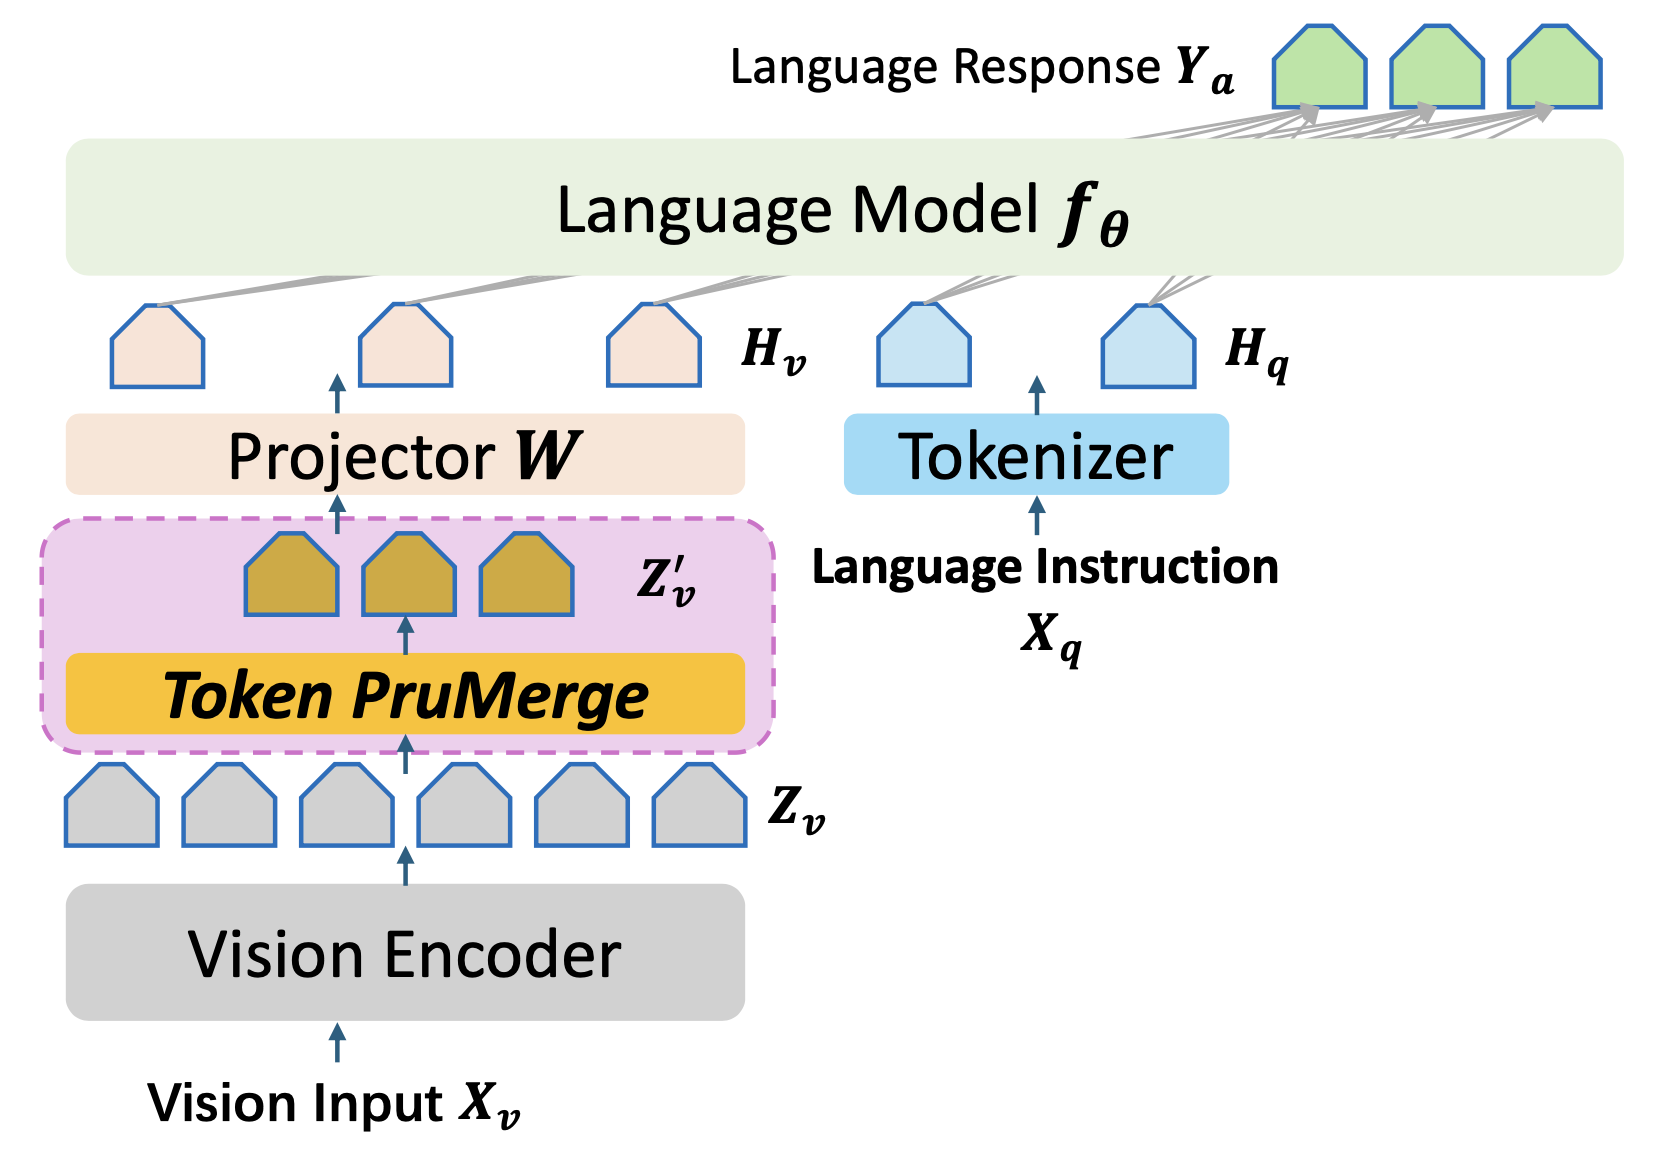
\includegraphics[width=0.6\textwidth]{images/purmerge-architecture.png}
    \caption{Schema of LLaVA-PruMerge \cite{shang2024LLaVA-PruMerge}}
    \label{fig:llava-prumerge-schema}
\end{figure}

\subsection{LLaVA-PruMerge}
To reduce the number of visual tokens, the authors of \cite{shang2024LLaVA-PruMerge} propose a method to merge visual tokens. The idea is to merge similar visual tokens and remove outliers. The process consists of the following steps:

\begin{itemize}
    \item \textbf{Class-Visual Attention}: First, the authors compute the attention between the class token and the visual tokens using the following formula:
    \begin{equation}
        a_{cls} = \text{softmax}\left(\frac{q_{cls} K^T}{\sqrt{d_k}}\right)
        \label{eq:attention}
    \end{equation}
    Here, $q_{cls}$ represents the query vector of the class token, $K$ is the key matrix of the visual tokens, and $d_k$ is the dimensionality of the key vectors.
    
    \item \textbf{Outlier Removal}: The authors remove outlier visual tokens using the Interquartile Range (IQR) method. Specifically, they calculate the difference between the 75th percentile and the 25th percentile of the attention weights. Visual tokens with attention weights more than 1.5 times the IQR below the 25th percentile or above the 75th percentile are identified as outliers and removed.
    
    \item \textbf{Merging}: The authors merge similar visual tokens using a k-nearest neighbors (k-NN) algorithm. For each selected token, they find the $k$ most similar visual tokens (including both selected and unselected tokens). They then compute a weighted sum of these tokens to create a new, merged token.
    
    \item \textbf{Token Supplement}: To address potential over-aggressiveness in token removal, the authors propose a token supplement step. They identify similarities between tokens using their “key” vectors (from the transformer’s self-attention mechanism). Pruned tokens are grouped with the most relevant retained tokens, which act as cluster centers. These pruned tokens are then merged into the clusters through a weighted averaging process, enriching the retained tokens with additional information.
\end{itemize}

The algorithm for LLaVA-PruMerge is presented in Algorithm~\ref{alg:prumerge}, and its architecture is illustrated in Figure~\ref{fig:llava-prumerge}.
\\
\\
\begin{algorithm}[H]
    \SetAlgoLined
    \caption{Token \textsc{PruMerge} algorithm for reducing the number of visual tokens. \cite{shang2024LLaVA-PruMerge}}
    \KwIn{Key and Query matrices of ViT's penultimate layer, $\mathbf{K} = \{\mathbf{k}_1, \cdots, \mathbf{k}_n\}$ and $\mathbf{Q} = \{\mathbf{q}_1, \cdots, \mathbf{q}_n\}$. The penultimate layer's output tokens, $\mathbf{Y} = \{\mathbf{y}_1, \cdots, \mathbf{y}_n\}$, where $n$ is the number of input visual tokens.}
    \KwOut{Refined $\mathbf{Y}$ to $m$ (adaptive) visual tokens $\mathbf{Y}' = \{\mathbf{y}'_1, \cdots, \mathbf{y}'_m\}$, where $m \ll n$.}
    
    \textbf{Token \textsc{PruMerge}:}
    
    \begin{enumerate}
        \item Calculate attention between visual token and class token $a_{[\text{cls}]}$ using Equation \ref{eq:attention}.
        \item Use the outlier detection algorithm IQR to adaptively select $m$ important visual tokens' indices $\{i_1, \cdots, i_m\}$ based on $a_{[\text{cls}]}$.
        \item \For{$p \in \{i_1, \cdots, i_m\}$}{
            Calculate the distance between selected token $\mathbf{y}_p$ and other visual tokens, $\mathbf{y}_{\{1, \cdots, n\} \setminus p}$\;
            Use $\mathbf{y}_p$ as the cluster center and run $k$-nearest neighbor algorithm to find $k$ similar tokens with indices $\{j_1, \cdots, j_k\}_p$\;
            Update cluster center token with weighted sum: $\mathbf{y}'_p = \sum_{q=1}^{k} a[j_q] \cdot \mathbf{y}_{j_q}$\;
        }
        \item Token supplement: find the k-nearest neighbors of the unpruned tokens and merge them back into the clusters using their similarity score as the metric where the similarity score is calculated using the dot product of the key vectors.
        \item Output a refined stack of visual tokens $\mathbf{Y}' = \{\mathbf{y}'_1, \cdots, \mathbf{y}'_m\}$.
    \end{enumerate}
    \label{alg:prumerge}    
\end{algorithm}

\begin{figure}[H]
    \centering
    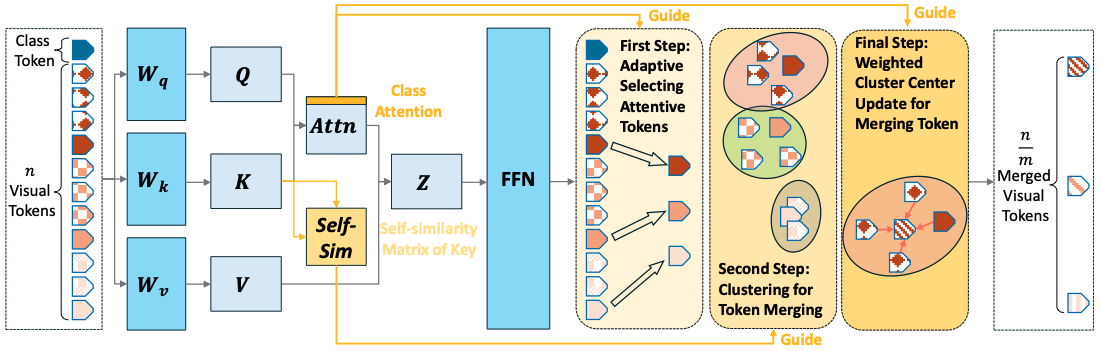
\includegraphics[width=0.8\textwidth]{images/prumerge.png}
    \caption{LLaVA-PruMerge architecture \cite{shang2024LLaVA-PruMerge}}
    \label{fig:llava-prumerge}
\end{figure}

\subsection{Experimentation and results}
To measure the efficiency of LLaVA-PruMerge, we planned to submit a set of images and prompts to both LLaVA and LLaVA-PruMerge and compare the time taken to generate outputs. Additionally, we intended to compare the outputs of both models to evaluate if their performance was similar.  

For a fair comparison, we chose to use the 7B versions of both models. Since LLaVA-PruMerge models are only available with LoRA, we ensured consistency by using LoRA for both models.  

Unfortunately, due to technical issues, we were unable to set up LLaVA (and consequently LLaVA-PruMerge) on our local machines. Despite extensive efforts on both macOS and Linux systems with GPU-enabled machines over several days, the setup was unsuccessful.  

As a result, we rely on the experimental results reported in \cite{shang2024LLaVA-PruMerge}. In their experiments, the authors compared the performance of LLaVA and LLaVA-PruMerge (along with other models) in their default versions and fine-tuned versions (trained for one epoch using LoRA) across multiple benchmarks. The results are presented in Table~\ref{tab:prumerge-results}.


\begin{table}[H]
    \centering
    \begin{tabular}{|c|c|c|c|c|c|c|}
        \hline
        Model & VQAv2 \cite{goyal2017making} & ScienceQA \cite{lu2022learn} & TextVQA \cite{singh2019towards} & POPE \cite{li2023evaluating} & MME \cite{yin2024survey} & MMBench \cite{liu2025mmbench}\\
        \hline
        LLaVA & 78.5 & 66.8 & 58.4 & 85.9 & 1510.7 & 60.9 \\
        LLaVA-PruMerge & 72.0 & 68.5 & 56.0 & 86.3 & 1350.3 & 60.9 \\
        LLaVA (fine-tuned) & 80.0 & 71.6 & 61.3 & 85.9 & 1531.3 & 67.7 \\
        LLaVA-PruMerge (fine-tuned) & 72.8 & 71.0 & 58.4 & 86.2 & 1428.2 & 62.3 \\
        \hline
    \end{tabular}
    \caption{Results of LLaVA and LLaVA-PruMerge on different benchmarks \cite{shang2024LLaVA-PruMerge}}
    \label{tab:prumerge-results}
\end{table}

We observe that LLaVA-PruMerge achieves performance comparable to LLaVA on most benchmarks. Notably, it outperforms LLaVA on ScienceQA and POPE benchmarks.  

In terms of efficiency, the results are summarized in Table~\ref{tab:prumerge-efficiency}.

\begin{table}[H]
    \centering
    \begin{tabular}{|c|c|c|c|c|c|c|}
        \hline
        Method & LLM Backbone & Quantization & FLOPs (T) \\
        \hline
        LLAVA-1.5 & Vicuna-7B & FP16 & 9.3 \\
        LLAVA-1.5 w/ PruMerge & Vicuna-7B & FP16 & 0.91 \\
        LLAVA-1.5 & Vicuna-7B & INT4 & 2.3  \\
        LLAVA-1.5 w/ PruMerge & Vicuna-7B & INT4 & 0.28 \\
        LLAVA-1.5 & Vicuna-13B & FP16 & 18.2  \\
        LLAVA-1.5 w/ PruMerge & Vicuna-13B & FP16 & 1.80 \\
        LLAVA-1.5 & Vicuna-13B & INT4 & 4.6   \\
        LLAVA-1.5 w/ PruMerge & Vicuna-13B & INT4 & 0.45 \\
        \hline
    \end{tabular}
    \caption{Efficiency of LLaVA and LLaVA-PruMerge on different benchmarks \cite{shang2024LLaVA-PruMerge}}
    \label{tab:prumerge-efficiency}
\end{table}
We observe that LLaVA-PruMerge is significantly more efficient than LLaVA. The number of FLOPs is reduced by approximately a factor of 10 when using LLaVA-PruMerge, representing a substantial improvement in efficiency.

\section{Conclusion}
In this report, we presented the LLaVA model and its efficiency enhancement, LLaVA-PruMerge. We discussed the key concepts behind LLaVA, its technical contributions, areas for improvement, and the LLaVA-PruMerge method. We then presented the results of LLaVA-PruMerge across various benchmarks and compared its efficiency to LLaVA. We found that LLaVA-PruMerge offers much greater efficiency than LLaVA while maintaining comparable performance. This represents a significant advancement in efficiency.

\bibliographystyle{plain}
\bibliography{mybibliography}

\appendix
The plagiarism detection score is approximately 26\%. Upon reviewing the report, it appears that the majority of the detected plagiarism comes from the references section. Therefore, excluding the references, the plagiarism score is around 13\%, which is acceptable. I hereby declare that this report is my own work and that I have not used any sources other than those cited in the references section.


% \section{Annex}
% \subsection{DataDAM code}
% \label{sec:DataDAM_code}
% Code for the DataDAM class. Mainly inspired from \cite{githubGitHubDataDistillationDataDAM}.
% \lstinputlisting{../DataDAM.py}
% \subsection{PAD code}
% \label{sec:PAD_code}
% Code for the PAD class. Partly inspired from \cite{githubGitHubNUSHPCAILabPAD}.
% \lstinputlisting{../PAD.py}
\end{document}
